\documentclass[fleqn,11pt]{article}

	\usepackage[letterpaper,margin=0.75in]{geometry}
	
	\usepackage{amsmath}
	\usepackage{booktabs}
	\usepackage{graphicx}
	\usepackage{listings}
	
	\setlength{\parindent}{1.4em}
	
	\begin{document}
	
	\lstset{
	  language=Python,
	  basicstyle=\small,          % print whole listing small
	  keywordstyle=\bfseries,
	  identifierstyle=,           % nothing happens
	  commentstyle=,              % white comments
	  stringstyle=\ttfamily,      % typewriter type for strings
	  showstringspaces=false,     % no special string spaces
	  numberstyle=\tiny,
	  numbersep=5pt,
	  frame=tb,
	}
	
	\title{Network Routing}
	
	\author{Chris Johnson}
	
	\date{19 March 2018}
	
	\maketitle
	
	\section{Test 1}
	
	First, the routing application was run over a simple, linear network to ensure that the forwarding
	tables would be constructed correctly. After the forwarding tables were filled, a packet was sent along
	the network, from one end to the other, to demonstrate that routing had worked correctly. 
	The network consisted of five nodes, n1
	through n5, each arranged in numerical order along a line. The nodes were connected by two-way links, with
	a bandwidth of 1 Mbps and a propagation delay of 1 ms. Each node broadcasted their distance vector once
	every second. When a distance vector was received, the node updated its own distance vector, and printed out
	the new distance vector.
	
	\subsection{results}
	
	The data below has two parts, the distance vector of n2 at each step in its construction and the trace of the
	packet sent from n1 to n5.
	
	\subsubsection{Node 2 Distance Vectors}
	
	\begin{enumerate}
	\item 0 seconds
\begin{lstlisting}
address: 2	distance: 0
address: 3	distance: 0
\end{lstlisting}
	
	\item 0.001 seconds
	
\begin{lstlisting}
address: 1	distance: 1
address: 2	distance: 0
address: 3	distance: 0
\end{lstlisting}
	 
	 \item 0.001 seconds
	 
\begin{lstlisting}
address: 1	distance: 1
address: 2	distance: 0
address: 3	distance: 0
address: 4	distance: 1
address: 5	distance: 1
\end{lstlisting}

	\item 1.001 seconds
	
\begin{lstlisting}
address: 1	distance: 1
address: 2	distance: 0
address: 3	distance: 0
address: 4	distance: 1
address: 5	distance: 1
address: 6	distance: 2
address: 7	distance: 2
\end{lstlisting}
	
	\item 2.001 seconds
	
\begin{lstlisting}
address: 1	distance: 1
address: 2	distance: 0
address: 3	distance: 0
address: 4	distance: 1
address: 5	distance: 1
address: 6	distance: 2
address: 7	distance: 2
address: 8	distance: 3
\end{lstlisting}
	
	\end{enumerate}
	
	\subsubsection{Packet Trace}
	
\begin{lstlisting}
3.2 n1 forwarding packet to 8
3.209 n2 forwarding packet to 8
3.218 n3 forwarding packet to 8
3.227 n4 forwarding packet to 8
3.236 n5 received packet
\end{lstlisting}
	
	\subsection{Analysis}
	
	The various distance vectors of n2 serve to show the process by which it was created as n2 received
	broadcasted distance vectors. At the first step, before any nodes have sent their distance vectors, there are
	only two entries. The second node owns addresses 2 and 3, so the only entries in its distance vector will be those addresses with a distance of 0, since they point to n2. After 0.1 seconds, each node has broadcasted its initial 
	distance vector. Step 2 shows the change made when n2 received the distance
	vector from n1, which only has one address, address 1. It is adjacent to n2, so the distance is 1. At the same time,
	n2 also received n3's distance vector, which is its other neighbor, so the distance to n3's addresses is also
	1. One second later, n3 broadcasts a distance vector that includes the distance to n4. n2 updates its distance vector
	with n4's addresses, 6 and 7. Finally, at 2.1 seconds, n2 is notified of the distance to n5, 3 hops.
	
	The second part of the results from this test simply show that the packet sent from n1 to n5, being forwarded by
	each node along the path. This shows that each node was able to properly build its forwarding table in order to
	transmit a packet along the length of the network.
	
	\section{Test 2}
	
	The second test shows how the routing application handles changes in the network. In this test, a similar network
	was used, except n1 and n5 are also linked biderectionally. This meant that the nodes formed a ring, where each node had two paths to any other node. Like the previous test, after the forwarding tables
	were built, a packet was sent along the network, this time from n2 to n3. Then, the link between n2 and n3 was
	disabled. After a few seconds, another packet was sent from n2 to n3 to show that the routing could handle
	changes in the network structure. To give the routing some time to account for the broken link, this second
	packet was sent 5 seconds after the link was taken down.
	
	
	\subsection{Results}
	
	{
		\subsubsection{Node 2 Distance Vectors}
		The distance vectors below show the steps that occur from the time that the forwarding table is initially filled
		to when the forwarding table accounts correctly for the link that was taken down.
		
		\vspace{.3cm}
		
		\begin{enumerate}
			\item 1.001 seconds
			
\begin{lstlisting}
address: 1	distance: 1
address: 2	distance: 1
address: 3	distance: 0
address: 4	distance: 0
address: 5	distance: 1
address: 6	distance: 1
address: 7	distance: 2
address: 8	distance: 2
address: 9	distance: 2
address: 10	distance: 2
\end{lstlisting}

			\item 5.001 seconds

\begin{lstlisting}
address: 1	distance: 1
address: 2	distance: 1
address: 3	distance: 0
address: 4	distance: 0
address: 5	distance: 4
address: 6	distance: 4
address: 7	distance: 3
address: 8	distance: 3
address: 9	distance: 2
address: 10	distance: 2
\end{lstlisting}

		\end{enumerate}
		
		\subsubsection{Packet Traces}
		The packet traces here show the two different paths taken, first when there is a link between n2 and n3, and then
		after that link is disabled.
		
		\begin{enumerate}
			\item Packet 1 - n2 to n3
		
\begin{lstlisting}
1.2 n2 forwarding packet to 5
1.209 n3 received packet
\end{lstlisting}

			\item Packet 2 - n2 to n3

\begin{lstlisting}
6.6 n2 forwarding packet to 5
6.609 n1 forwarding packet to 5
6.618 n5 forwarding packet to 5
6.627 n4 forwarding packet to 5
6.636 n3 received packet
\end{lstlisting}

		\end{enumerate}
	}

	\subsection{Analysis}
	
	The distance vector of n2 is almost identical to the first test, but the distance to node 5 is shorter, since
	n2 can transmit to n5 through n1. After the link between n2 and n3 gets taken down, there is a three second delay until
	n2 registers the change. It takes a few more iterations for the distance vector to become fully updated, but the
	result is shown in the second distance vector. The most obvious change is that instead of a distance of 1, the
	distance from n2 to the addressed of n3 is now 4, since they no longer share a link.
	
	This is also reflected in the path taken by the packet in both cases. The single hop from n2 to n3 for the first
	packet becomes 4 hops. This trace also shows that the forwarding table at n1 also updated properly. Before the link
	was taken down, the fastest path to n3 from n1 was through n2. Without the n2-n3 link, however, this was obviously
	no longer the case, and n1 began to route packets for n3 through n5.
	
	\section{Test 3}
	
	The network used for the final test was much more complex than the previous two configurations. It consisted
	of 15 nodes with varying levels of connectivity between them. The configuration is represented in the
	following graph structure:
	
	\begin{center}
		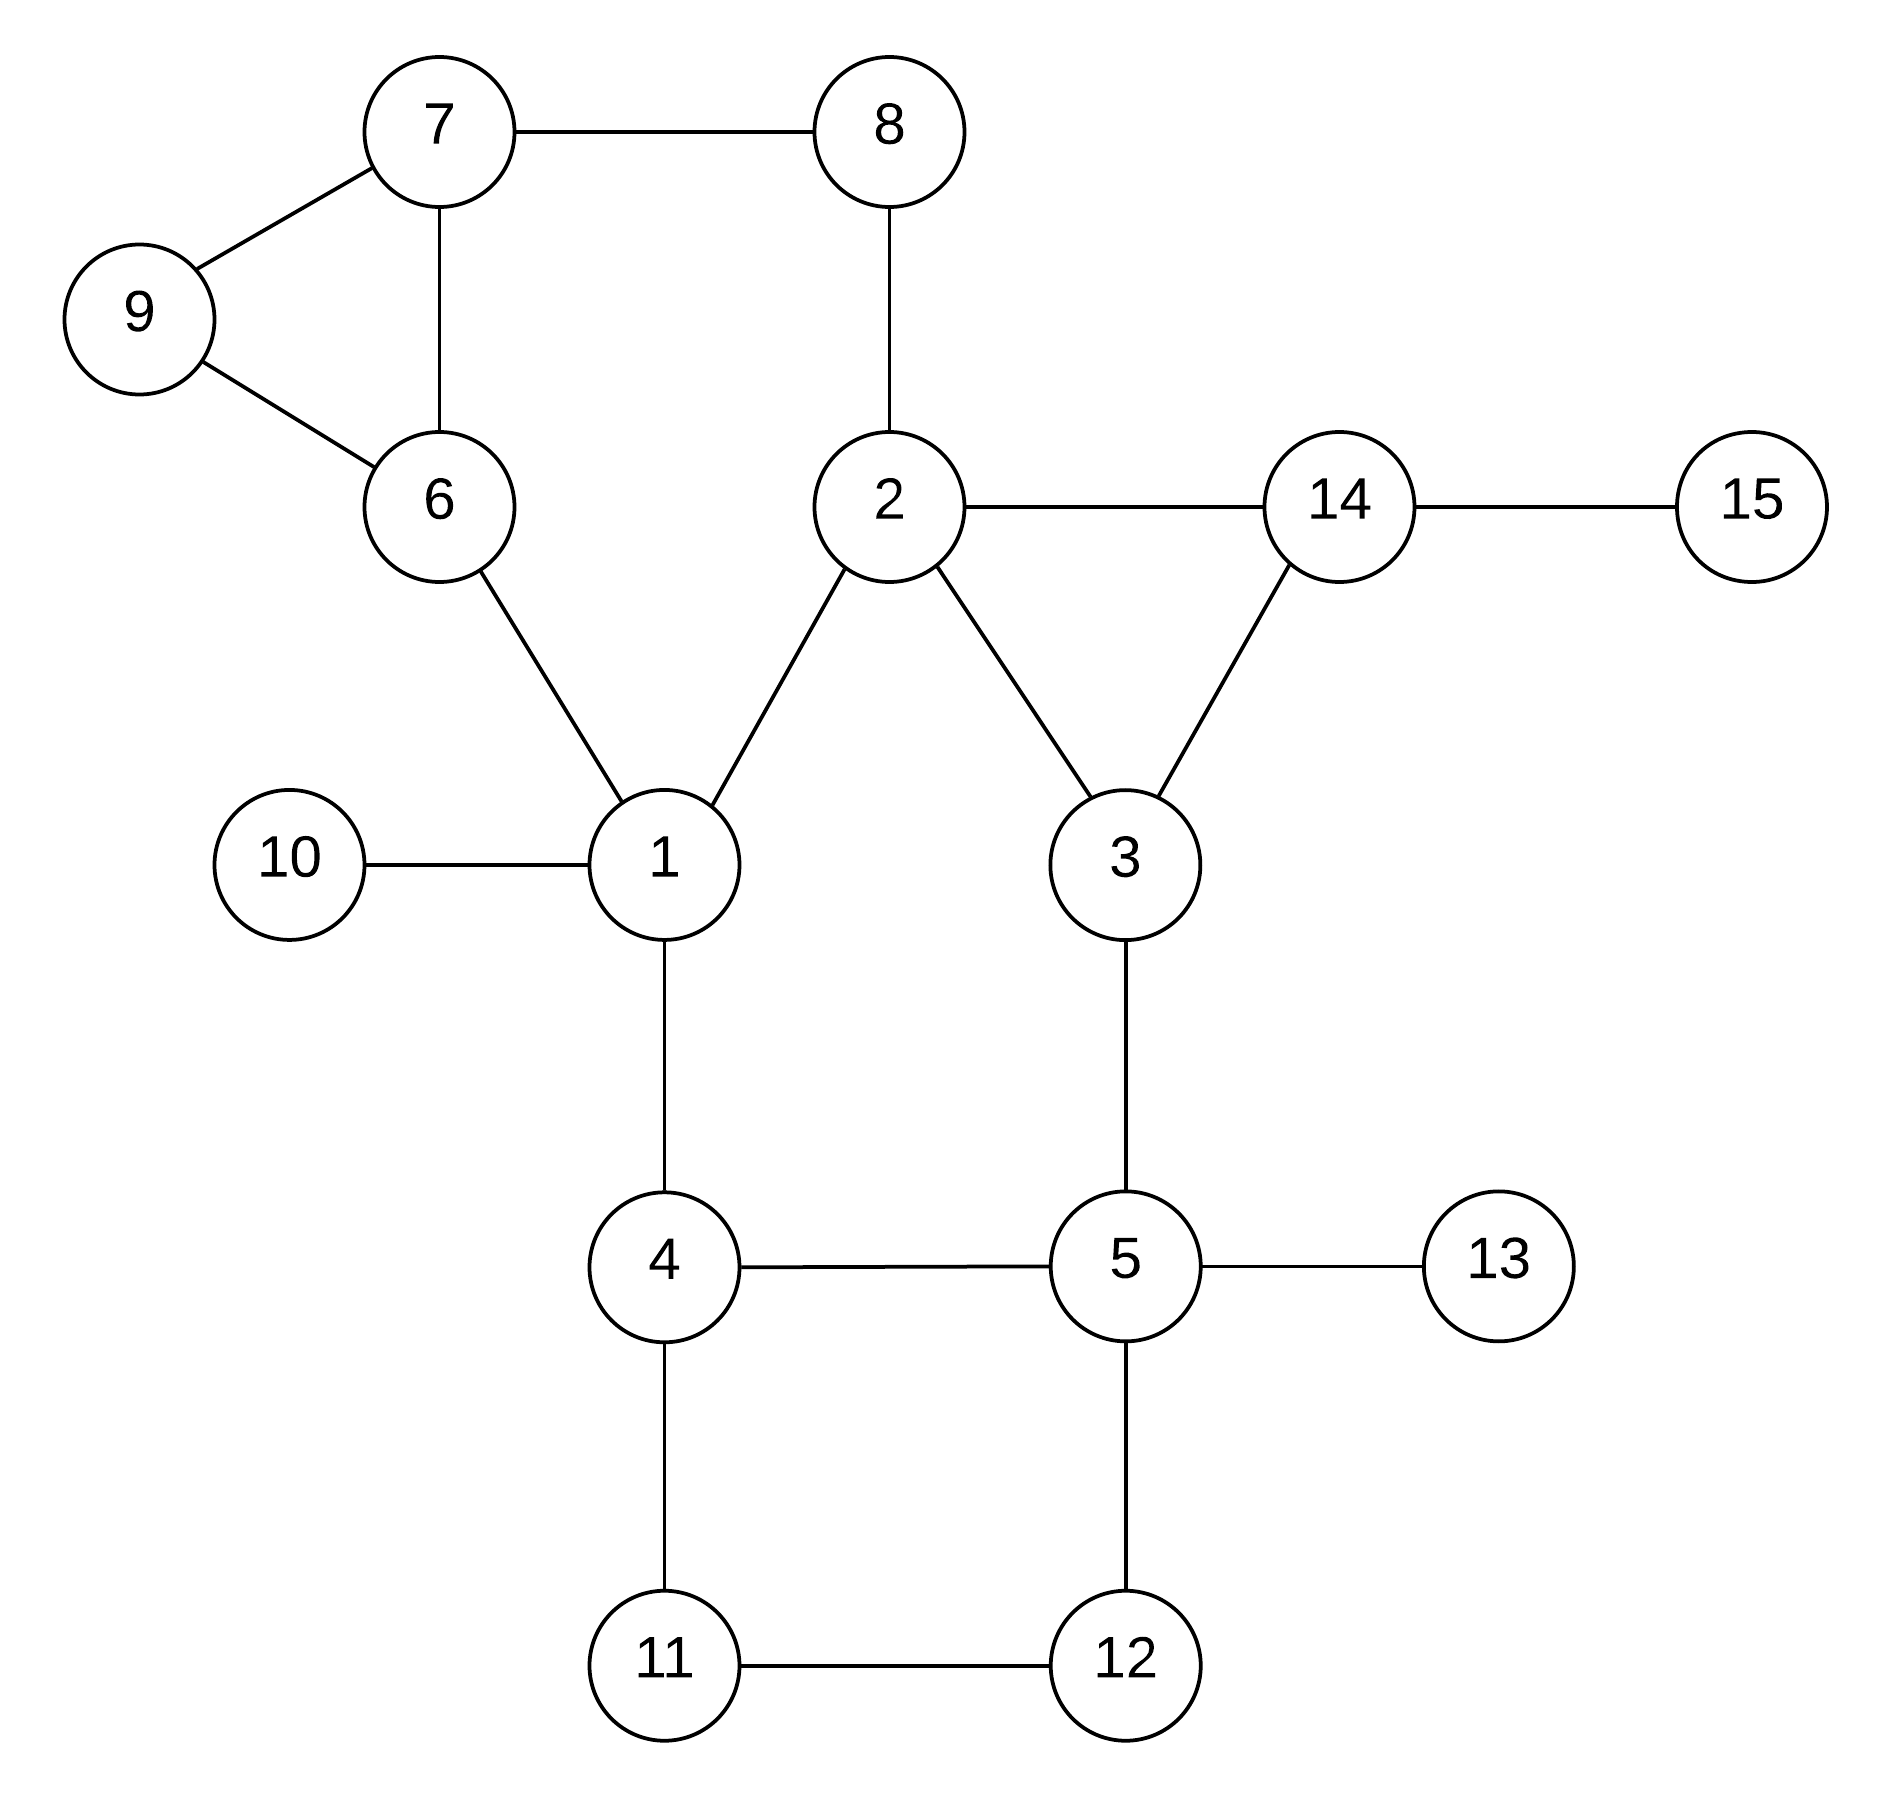
\includegraphics[width=10cm]{15nodes}
	\end{center}
		
	In this test, after the routing algorithm finished, several packets were sent to demonstrate that
	routing worked correctly. A packet was transmitted from n11 to n15, from n12 to n7, and from n8 to n10.
	Then the link between n8 and n2 was taken down. A packet was again sent from node 8 to node 10. This time
	the link was brought back up, and another packet was sent on the same path, n8 to n10. This served
	to demonstrate that the routing application could handle both changes in the network structure. Not
	only does the distance vector algorithm respond correctly to a link being removed, but it also accounts
	for links being added that create a shorter path.
	
	\subsection{Results}
	
		\subsubsection{Node 8 distance vectors}
		\begin{enumerate}
			\item 3.001 seconds
			
\begin{lstlisting}
address: 1	distance: 2
address: 2	distance: 2
address: 3	distance: 2
address: 4	distance: 2
address: 5	distance: 1
address: 6	distance: 1
address: 7	distance: 1
address: 8	distance: 1
address: 9	distance: 2
address: 10	distance: 2
address: 11	distance: 2
address: 12	distance: 3
address: 13	distance: 3
address: 14	distance: 3
address: 15	distance: 3
address: 16	distance: 3
address: 17	distance: 3
address: 18	distance: 3
address: 19	distance: 2
address: 20	distance: 2
address: 21	distance: 2
address: 22	distance: 1
address: 23	distance: 1
address: 24	distance: 1
address: 25	distance: 0
address: 26	distance: 0
address: 27	distance: 2
address: 28	distance: 2
address: 29	distance: 3
address: 30	distance: 4
address: 31	distance: 4
address: 32	distance: 4
address: 33	distance: 2
address: 34	distance: 2
address: 35	distance: 2
address: 36	distance: 3
\end{lstlisting}

		\item 10.001 seconds
		
\begin{lstlisting}
address: 1	distance: 3
address: 2	distance: 3
address: 3	distance: 3
address: 4	distance: 3
address: 5	distance: 3
address: 6	distance: 3
address: 7	distance: 3
address: 8	distance: 3
address: 9	distance: 4
address: 10	distance: 4
address: 11	distance: 4
address: 12	distance: 4
address: 13	distance: 4
address: 14	distance: 4
address: 15	distance: 5
address: 16	distance: 5
address: 17	distance: 5
address: 18	distance: 5
address: 19	distance: 2
address: 20	distance: 2
address: 21	distance: 2
address: 22	distance: 1
address: 23	distance: 1
address: 24	distance: 1
address: 25	distance: 0
address: 26	distance: 0
address: 27	distance: 2
address: 28	distance: 2
address: 29	distance: 4
address: 30	distance: 5
address: 31	distance: 6
address: 32	distance: 6
address: 33	distance: 4
address: 34	distance: 4
address: 35	distance: 4
address: 36	distance: 5
\end{lstlisting}

		\item 16.001 seconds
		
\begin{lstlisting}
address: 1	distance: 2
address: 2	distance: 2
address: 3	distance: 2
address: 4	distance: 2
address: 5	distance: 1
address: 6	distance: 1
address: 7	distance: 1
address: 8	distance: 1
address: 9	distance: 2
address: 10	distance: 2
address: 11	distance: 2
address: 12	distance: 3
address: 13	distance: 3
address: 14	distance: 3
address: 15	distance: 3
address: 16	distance: 3
address: 17	distance: 3
address: 18	distance: 3
address: 19	distance: 2
address: 20	distance: 2
address: 21	distance: 2
address: 22	distance: 1
address: 23	distance: 1
address: 24	distance: 1
address: 25	distance: 0
address: 26	distance: 0
address: 27	distance: 2
address: 28	distance: 2
address: 29	distance: 3
address: 30	distance: 4
address: 31	distance: 4
address: 32	distance: 4
address: 33	distance: 2
address: 34	distance: 2
address: 35	distance: 2
address: 36	distance: 3
\end{lstlisting}

		\end{enumerate}
	
		\subsubsection{Packet Traces}
		
		\begin{enumerate}
			\item Packet 1 - n12 to n7
\begin{lstlisting}
4.2 n12 forwarding packet to 22
4.209 n5 forwarding packet to 22
4.218 n3 forwarding packet to 22
4.227 n2 forwarding packet to 22
4.236 n8 forwarding packet to 22
4.245 n7 received packet
\end{lstlisting}
			\item Packet 3 - n11 to n15
\begin{lstlisting}
4.3 n11 forwarding packet to 36
4.309 n4 forwarding packet to 36
4.318 n1 forwarding packet to 36
4.327 n2 forwarding packet to 36
4.336 n14 forwarding packet to 36
4.345 n15 received packet
\end{lstlisting}
			\item Packet 3 - n8 to n10
\begin{lstlisting}
4.4 n8 forwarding packet to 29
4.409 n2 forwarding packet to 29
4.418 n1 forwarding packet to 29
4.427 n10 received packet
\end{lstlisting}
			\item Packet 4 - n8 to n10
\begin{lstlisting}
10.4 n8 forwarding packet to 29
10.409 n7 forwarding packet to 29
10.418 n6 forwarding packet to 29
10.427 n1 forwarding packet to 29
10.436 n10 received packet
\end{lstlisting}	
			\item Packet 5 - n8 to n10
\begin{lstlisting}
16.4 n8 forwarding packet to 29
16.409 n2 forwarding packet to 29
16.418 n1 forwarding packet to 29
16.427 n10 received packet
\end{lstlisting}
					
		\end{enumerate}
	
	\subsection{Analysis}
	`
	The three distance vectors illustrate how the forwarding table of n8 changed as the link between n8 and n2 was
	deactivated and then enabled again. The most important part is the change of the distance to address 29. This
	address corresponds to n10. The fastest path from n8 to n10 initially is 3 hops, through the n8-n2 link. When that
	link is taken down, the fastest path is increased to 4 hops. The other distances show how removing one link affects
	the forwarding table of the entire network mesh.
	
	The initial packet traces demonstrate the correctness of the forwarding table. Each packet sent just after 4 seconds
	takes the path expected based on the network structure. This includes the packet sent from n8. It travels to n10 in 
	3 hops. After the n8-n2 link is taken down, however, packet 4 is sent from n8 to n10, and it now takes 4 hops. The
	fastest path is no longer available so the network adjusts and finds an alternative path. After the link is
	restored, it takes a few seconds for n8 to be notified of the fastest path, but it does select the link to n2 for
	the forwarding table. As expected, the path from n8 is exactly the same as in the initial network state.
	
	\end{document}
	